\documentclass{article}

\usepackage{fullpage}
\usepackage{amsmath}
\usepackage{amsfonts}
\usepackage{graphicx}
\usepackage{algorithmic}
\usepackage{xcolor}
\usepackage{framed}

\definecolor{dark_red}{rgb}{0.5,0.0,0.0}

\newcommand{\abs}[1]{\left|#1\right|}
\newcommand{\atan}{\text{atan}}
\newcommand{\rowvec}[3]{\left\langle #1, #2, #3 \right\rangle}
\newcommand{\colvec}[3]{\begin{bmatrix} #1 \\ #2 \\ #3 \end{bmatrix}}
\newcommand{\at}[1]{\left. #1 \right|}
\newcommand{\diff}[2]{\frac{d #1}{d #2}}
\newcommand{\partdiff}[2]{\frac{\partial #1}{\partial #2}}
\newcommand{\mvec}[1]{\overrightarrow{\mathbf{#1}}}
\newcommand{\pvec}[1]{\overrightarrow{#1}}
\newcommand{\dr}[1]{\textcolor{dark_red}{#1}}


\title{Cartesian and Polar Double Integrals}
\date{}

\begin{document}

\maketitle




%%%%%%%%%%%%%%%%%% QUESTION 1
\section*{Question 1:}

\subsection*{part 1a:}

For the following double integrals, convert the function that is being integrated over (the integrand) from a function of Cartesian coordinates to a function of Polar coordinates:

\begin{itemize}
\item \(\iint_{\sigma} (x + y)dA\)
\item \(\iint_{\sigma} xy dA\)
\item \(\iint_{\sigma} \frac{y}{x}dA\)
\item \(\iint_{\sigma} \frac{dA}{(x^2 + y^2)^{3/2}}\)
\item \(\iint_{\sigma} \frac{x^2 - y^2}{2xy} dA\)
\end{itemize}

%%%%%%%%%%%%%%%%%% SOLUTION 1A

\vspace{5mm}
\dr{\textbf{Solution:}}

\dr{
\begin{itemize}
\item \(\iint_{\sigma} (x + y)dA = \iint_{\sigma} (r\cos\theta + r\sin\theta)dA = \iint_{\sigma} r(\cos\theta + \sin\theta)dA\)
\item \(\iint_{\sigma} xy dA = \iint_{\sigma} (r\cos\theta)(r\sin\theta) dA = \iint_{\sigma} \frac{1}{2}r^2\sin(2\theta) dA\)
\item \(\iint_{\sigma} \frac{y}{x}dA = \iint_{\sigma} \frac{r\sin\theta}{r\cos\theta}dA = \iint_{\sigma} \tan\theta dA\)
\item \(\iint_{\sigma} \frac{dA}{(x^2 + y^2)^{3/2}} = \iint_{\sigma} \frac{dA}{(r^2\cos^2\theta + r^2\sin^2\theta)^{3/2}} = \iint_{\sigma} \frac{dA}{r^3}\)
\item \(\iint_{\sigma} \frac{x^2 - y^2}{2xy} dA = \iint_{\sigma} \frac{r^2\cos^2\theta - r^2\sin^2\theta}{2(r\cos\theta)(r\sin\theta)} dA = \iint_{\sigma} \frac{\cos(2\theta)}{\sin(2\theta)} dA = \iint_{\sigma} \cot(2\theta) dA\)
\end{itemize}
}


\subsection*{part 1b:}

For the following double integrals, convert the function that is being integrated over (the integrand) from a function of Polar coordinates to a function of Cartesian coordinates:

\begin{itemize}
\item \(\iint_{\sigma} r\cos\theta dA\)
\item \(\iint_{\sigma} r^2\sin\theta dA\)
\item \(\iint_{\sigma} r^{-3}dA\)
\item \(\iint_{\sigma} \frac{\cos\theta - 3\sin\theta}{2\cos\theta + \sin\theta}dA\)
\item \(\iint_{\sigma} r\tan\theta dA\)
\item \(\iint_{\sigma} \cos(2\theta) dA\)
\item \(\iint_{\sigma} \sin(2\theta) dA\)
\item \(\iint_{\sigma} \tan(2\theta) dA\)
\end{itemize}

%%%%%%%%%%%%%%%%%% SOLUTION 1B

\vspace{5mm}
\dr{\textbf{Solution:}}

\dr{
\begin{itemize}
\item \(\iint_{\sigma} r\cos\theta dA = \iint_{\sigma} r(x/r) dA = \iint_{\sigma} x dA\)
\item \(\iint_{\sigma} r^2\sin\theta dA = \iint_{\sigma} r^2(y/r) dA = \iint_{\sigma} yr dA = \iint_{\sigma} y\sqrt{x^2 + y^2} \cdot dA\)
\item \(\iint_{\sigma} r^{-3}dA = \iint_{\sigma} \frac{1}{(x^2 + y^2)^{3/2}}dA\)
\item \(\iint_{\sigma} \frac{\cos\theta - 3\sin\theta}{2\cos\theta + \sin\theta}dA = \iint_{\sigma} \frac{x/r - 3(y/r)}{2(x/r) + y/r}dA = \iint_{\sigma} \frac{x - 3y}{2x + y}dA\)
\item \(\iint_{\sigma} r\tan\theta dA = \iint_{\sigma} r(y/x) dA = \iint_{\sigma} \frac{y\sqrt{x^2 + y^2}}{x} dA\)
\item \(\iint_{\sigma} \cos(2\theta) dA = \iint_{\sigma} (\cos^2\theta - \sin^2\theta)dA = \iint_{\sigma} ((x/r)^2 - (y/r)^2)dA = \iint_{\sigma} \frac{x^2 - y^2}{r^2}dA = \iint_{\sigma} \frac{x^2 - y^2}{x^2 + y^2}dA\)
\item \(\iint_{\sigma} \sin(2\theta) dA = \iint_{\sigma} 2\cos\theta\sin\theta dA = \iint_{\sigma} 2(x/r)(y/r) dA = \iint_{\sigma} \frac{2xy}{r^2} dA = \iint_{\sigma} \frac{2xy}{x^2 + y^2} dA\)
\item \(\iint_{\sigma} \tan(2\theta) dA = \iint_{\sigma} \frac{\sin(2\theta)}{\cos(2\theta)} dA = \iint_{\sigma} \frac{2\cos\theta\sin\theta}{\cos^2\theta - \sin^2\theta} dA = \iint_{\sigma} \frac{2(x/r)(y/r)}{(x/r)^2 - (y/r)^2} dA = \iint_{\sigma} \frac{2xy}{x^2 - y^2} dA\)
\end{itemize}
}




%%%%%%%%%%%%%%%%%% QUESTION 2
\section*{Question 2:}

\subsection*{part 2a:}

For the following regions characterized using Cartesian coordinates, express these regions using Polar coordinates:

\begin{itemize}
\item \(\sigma = \{(x,y) | -2 \leq x \leq 2 \;\text{and}\; 0 \leq y \leq \sqrt{4 - x^2}\}\)
\item \(\sigma = \{(x,y) | 0 \leq x \leq 2 \;\text{and}\; -\sqrt{4 - x^2} \leq y \leq \sqrt{4 - x^2}\}\)
\item \(\sigma = \{(x,y) | 0 \leq x \leq 1 \;\text{and}\; -\frac{x}{\sqrt{3}} \leq y \leq x\}\)
\item \(\sigma = \{(x,y) | -2 \leq x \leq 2 \;\text{and}\; 0 \leq y \leq 4 - x^2\}\)
\item \(\sigma = \{(x,y) | 0 \leq y \leq 3 \;\text{and}\; -5 + (5/3)y \leq x \leq 0\}\)
\item \(\sigma = \{(x,y) | -1 \leq x \leq 1 \;\text{and}\; 1 - \sqrt{1 - x^2} \leq y \leq 1 + \sqrt{1 - x^2}\}\)
\item \(\sigma = \{(x,y) | 1 - \sqrt{2} \leq x \leq 1 + \sqrt{2} \;\text{and}\; 1 - \sqrt{-x^2 + 2x + 1} \leq y \leq 1 + \sqrt{-x^2 + 2x + 1}\}\)
\item \(\sigma = \{(x,y) | -6 \leq x \leq 0 \;\text{and}\; 2x^2 + 12x \leq y \leq 0\}\)
\end{itemize}

%%%%%%%%%%%%%%%%%% SOLUTION 2A

\vspace{5mm}
\dr{\textbf{Solution:}}

%1
\dr{\begin{framed}
For \(\sigma = \{(x,y) | -2 \leq x \leq 2 \;\text{and}\; 0 \leq y \leq \sqrt{4 - x^2}\}\), \\
\begin{tabular}{cc}
\parbox{0.6\textwidth}{
The region can easily be plotted on the right. \\
The curve \(y = \sqrt{4 - x^2}\) is equivalent to:
\begin{align*}
y = \sqrt{4 - x^2} \implies & y^2 = 4 - x^2 
\iff r^2\sin^2\theta = 4 - r^2\cos^2\theta \\
\iff & r^2 = 4 
\iff r = 2 
\end{align*}
\(r = 2\), along with \(y \geq 0\), gives the region \(\sigma\) on the right:
} & \parbox{0.4\textwidth}{

\includegraphics[width = 0.4\textwidth]{Test_bench_part_3x_images/Test_bench_part_3x_Solutions_image_1}
} 
\end{tabular} \\
Therefore \(\sigma = \{(r,\theta) | 0 \leq \theta \leq \pi \;\text{and}\; 0 \leq r \leq 2\}\)
\end{framed}}


%2
\dr{\begin{framed}
For \(\sigma = \{(x,y) | 0 \leq x \leq 2 \;\text{and}\; -\sqrt{4 - x^2} \leq y \leq \sqrt{4 - x^2}\}\), \\
\begin{tabular}{cc}
\parbox{0.6\textwidth}{
The region can easily be plotted on the right. \\
The curve \(y = \pm\sqrt{4 - x^2}\) is equivalent to: 
\begin{align*}
y = \pm\sqrt{4 - x^2} \iff & y^2 = 4 - x^2 
\iff r^2\sin^2\theta = 4 - r^2\cos^2\theta \\
\iff & r^2 = 4 
\iff r = 2
\end{align*}
\(r = 2\), along with \(x \geq 0\), gives the region \(\sigma\) on the right:
} & \parbox{0.2\textwidth}{

\includegraphics[width = 0.2\textwidth]{Test_bench_part_3x_images/Test_bench_part_3x_Solutions_image_2}
}
\end{tabular} \\
Therefore \(\sigma = \left\{(r,\theta) \middle| -\frac{\pi}{2} \leq \theta \leq \frac{\pi}{2} \;\text{and}\; 0 \leq r \leq 2\right\}\)
\end{framed}}

\pagebreak

%3
\dr{\begin{framed}
For \(\sigma = \{(x,y) | 0 \leq x \leq 1 \;\text{and}\; -\frac{x}{\sqrt{3}} \leq y \leq x\}\), \\
\begin{tabular}{cc}
\parbox{0.6\textwidth}{
The region can easily be plotted on the right. \\
%The line \(y = -\frac{x}{\sqrt{3}}\) is equivalent to: 
%\begin{align*} 
%\theta = & \atan(-\frac{1}{\sqrt{3}}) \;\text{or}\; \pi + \atan(-\frac{1}{\sqrt{3}}) \\
%= & -\frac{\pi}{6} \;\text{or}\; \frac{5\pi}{6} 
%\end{align*}
%The line \(y = x\) is equivalent to \(\theta = \frac{\pi}{4}, -\frac{3\pi}{4}\) \\
The counterclockwise angle of line \(y = -\frac{x}{\sqrt{3}}\) relative to the positive \(x\)-axis is \(\atan(-\frac{1}{\sqrt{3}}) = -\frac{\pi}{6}\), so the lower bound on \(\theta\) is \(-\frac{\pi}{6}\). \\
The counterclockwise angle of line \(y = x\) relative to the positive \(x\)-axis is \(\atan(1) = \frac{\pi}{4}\), so the upper bound on \(\theta\) is \(\frac{\pi}{4}\). \\
The line \(x = 1\) is equivalent to:
\begin{align*}
x = 1 \iff & r\cos\theta = 1 
\iff r = \sec\theta
\end{align*}
%The former two lines give the bounds on \(\theta\), while the latter line gives the upper bound on \(r\). 
This line gives the upper bound on \(r\).
} & \parbox{0.4\textwidth}{

\includegraphics[width = 0.4\textwidth]{Test_bench_part_3x_images/Test_bench_part_3x_Solutions_image_3}
}
\end{tabular} \\
Therefore \(\sigma = \left\{(r,\theta) \middle| -\frac{\pi}{6} \leq \theta \leq \frac{\pi}{4} \;\text{and}\; 0 \leq r \leq \sec\theta\right\}\)
\end{framed}}


%4
\dr{\begin{framed}
For \(\sigma = \{(x,y) | -2 \leq x \leq 2 \;\text{and}\; 0 \leq y \leq 4 - x^2\}\), \\
\begin{tabular}{cc}
\parbox{0.6\textwidth}{
The region can easily be plotted on the right. \\
The curve \(y = 4 - x^2\) is equivalent to:
\begin{align*}
y = 4 - x^2 \iff & r\sin\theta = 4 - r^2\cos^2\theta \\
\iff & (\cos^2\theta)r^2 + (\sin\theta)r - 4 = 0 \\
\iff & r = \frac{-\sin\theta + \sqrt{\sin^2\theta + 16\cos^2\theta}}{2\cos^2\theta} \\
\iff & r = \frac{-\sin\theta + \sqrt{1 + 15\cos^2\theta}}{2\cos^2\theta}
\end{align*}
The other root is omitted since \(r\) must be nonnegative.
} & \parbox{0.4\textwidth}{
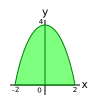
\includegraphics[width = 0.4\textwidth]{Test_bench_part_3x_images/Test_bench_part_3x_Solutions_image_4}
}
\end{tabular} \\
Therefore \(\sigma = \left\{(r,\theta) \middle| 0 \leq \theta \leq \pi \;\text{and}\; 0 \leq r \leq \frac{-\sin\theta + \sqrt{1 + 15\cos^2\theta}}{2\cos^2\theta} \right\}\)
\end{framed}}

\pagebreak

%5
\dr{\begin{framed}
For \(\sigma = \{(x,y) | 0 \leq y \leq 3 \;\text{and}\; -5 + (5/3)y \leq x \leq 0\}\), \\
\begin{tabular}{cc}
\parbox{0.6\textwidth}{
The region can easily be plotted on the right. \\
The line \(x = -5 + (5/3)y\) is equivalent to: 
\begin{align*}
x = -5 + (5/3)y \iff & r\cos\theta = -5 + \frac{5}{3}r\sin\theta \\
\iff & ((5/3)\sin\theta - \cos\theta)r = 5 \\
\iff & r = \frac{15}{5\sin\theta - 3\cos\theta}
\end{align*}
} & \parbox{0.4\textwidth}{
\includegraphics[width = 0.4\textwidth]{Test_bench_part_3x_images/Test_bench_part_3x_Solutions_image_5}
}
\end{tabular} \\
Therefore \(\sigma = \left\{(r,\theta) \middle| \frac{\pi}{2} \leq \theta \leq \pi \;\text{and}\; 0 \leq r \leq \frac{15}{5\sin\theta - 3\cos\theta}\right\}\)
\end{framed}}


%6
\dr{\begin{framed}
For \(\sigma = \{(x,y) | -1 \leq x \leq 1 \;\text{and}\; 1 - \sqrt{1 - x^2} \leq y \leq 1 + \sqrt{1 - x^2}\}\), \\
\begin{tabular}{cc}
\parbox{0.6\textwidth}{
The region can easily be plotted on the right. \\
The curve \(y = 1 \pm \sqrt{1 - x^2}\) is equivalent to:
\begin{align*}
& y = 1 \pm \sqrt{1 - x^2} 
\iff (y - 1)^2 = 1 - x^2 \\
\iff & y^2 - 2y + 1 = 1 - x^2 
\iff x^2 + y^2 - 2y = 0 \\
\iff & r^2\cos^2\theta + r^2\sin^2\theta - 2r\sin\theta = 0 
\iff r^2 = 2r\sin\theta \\
\iff & r = 0, 2\sin\theta
\end{align*} 
} & \parbox{0.4\textwidth}{
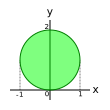
\includegraphics[width = 0.4\textwidth]{Test_bench_part_3x_images/Test_bench_part_3x_Solutions_image_6}
}
\end{tabular} \\
Therefore \(\sigma = \{(r,\theta) | 0 \leq \theta \leq \pi \;\text{and}\; 0 \leq r \leq 2\sin\theta\}\)
\end{framed}}

\pagebreak

%7
\dr{\begin{framed}
For \(\sigma = \{(x,y) | 1 - \sqrt{2} \leq x \leq 1 + \sqrt{2} \;\text{and}\; 1 - \sqrt{-x^2 + 2x + 1} \leq y \leq 1 + \sqrt{-x^2 + 2x + 1}\}\), \\
\begin{tabular}{cc}
\parbox{0.6\textwidth}{
The curve \(y = 1 \pm \sqrt{-x^2 + 2x + 1}\) is equivalent to: \\
\begin{align*}
& y = 1 \pm \sqrt{-x^2 + 2x + 1} 
\iff (y - 1)^2 = -x^2 + 2x + 1 \\
\iff & (x^2 - 2x) + (y - 1)^2 = 1 
\iff (x - 1)^2 + (y - 1)^2 = 2
\end{align*}
This curve is a circle centered on the point \((1,1)\) and has radius of \(\sqrt{2}\). The region \(\sigma\) is plotted on the right. \\
Converting the circle to polar coordinates gives: 
\begin{align*}
& (x - 1)^2 + (y - 1)^2 = 2 
\iff x^2 + y^2 - 2x - 2y = 0 \\
\iff & r^2\cos^2\theta + r^2\sin^2\theta - 2r\cos\theta - 2r\sin\theta = 0 \\
\iff & r^2 = 2r(\cos\theta + \sin\theta) 
\iff r = 0, 2(\cos\theta + \sin\theta) 
\end{align*}
The bounds for \(\theta\) can easily be determined from the drawing of \(\sigma\).
} & \parbox{0.4\textwidth}{
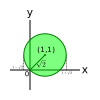
\includegraphics[width = 0.4\textwidth]{Test_bench_part_3x_images/Test_bench_part_3x_Solutions_image_7}
}
\end{tabular} \\
Therefore \(\sigma = \left\{(r,\theta) \middle| -\frac{\pi}{4} \leq \theta \leq \frac{3\pi}{4} \;\text{and}\; 0 \leq r \leq 2(\cos\theta + \sin\theta)\right\}\)
\end{framed}}

%7x
\dr{\begin{framed}
For \(\sigma = \{(x,y) | -6 \leq x \leq 0 \;\text{and}\; 2x^2 + 12x \leq y \leq 0\}\), \\
\begin{tabular}{cc}
\parbox{0.6\textwidth}{
The region \(\sigma\) can easily be plotted on the right, and is entirely contained in the \(-x,-y\) quadrant. \\
The curve \(y = 2x^2 + 12x\) is equivalent to: \\
\begin{align*}
& y = 2x^2 + 12x \\
\iff & r\sin\theta = 2r^2\cos^2\theta + 12r\cos\theta \\
\iff & r^2 = r\frac{\sin\theta - 12\cos\theta}{2\cos^2\theta} 
\iff r = 0, \frac{\sin\theta - 12\cos\theta}{2\cos^2\theta} 
\end{align*}
The lower bound for \(\theta\) is clearly \(-\pi\). The upper bound for \(\theta\) is determined by the angle that the parabola \(y = 2x^2 + 12x\) makes with the \(x\)-axis at the origin. At the origin, the parabola has a slope of \(12\), so the angle made with the \(x\)-axis is \(\atan(12)\). On the left side of the \(y\)-axis (\(x \leq 0\)), this angle induces the upper bound of \(-\pi + \atan(12)\) for \(\theta\).
} & \parbox{0.4\textwidth}{

\includegraphics[width = 0.4\textwidth]{Test_bench_part_3x_images/Test_bench_part_3x_Solutions_image_7x}
}
\end{tabular} \\
Therefore \(\sigma = \left\{(r,\theta) \middle| -\pi \leq \theta \leq -\pi + \atan(12) \;\text{and}\; 0 \leq r \leq \frac{\sin\theta - 12\cos\theta}{2\cos^2\theta}\right\}\)
\end{framed}}



%%%%%%%%%%%%%%%%%% SOLUTION 2B

\subsection*{part 2b:} 

For the following regions characterized using Polar coordinates, express these regions using Cartesian coordinates:

\begin{itemize}
\item \(\sigma = \left\{(r,\theta) \middle| -\frac{\pi}{2} \leq \theta \leq \frac{\pi}{4} \;\text{and}\; 0 \leq r \leq \frac{3}{2\cos\theta - \sin\theta}\right\}\)
\item \(\sigma = \left\{(r,\theta) \middle| 0 \leq \theta \leq \frac{\pi}{4} \;\text{and}\; 0 \leq r \leq 2\sin\theta\right\}\)
\item \(\sigma = \left\{(r,\theta) \middle| -\atan(2) \leq \theta \leq \frac{\pi}{4} \;\text{and}\; 0 \leq r \leq \frac{2\cos\theta + \sin\theta}{\cos^2\theta}\right\}\) 
\item \(\sigma = \left\{(r,\theta) \middle| -\frac{\pi}{2} \leq \theta \leq \atan(\frac{3}{2}) \;\text{and}\; 0 \leq r \leq \frac{\sin\theta + \sqrt{1 + 3\cos^2\theta}}{2\cos^2\theta}\right\}\)
\item \(\sigma = \left\{(r,\theta) \middle| -\frac{\pi}{6} \leq \theta \leq \frac{\pi}{6} \;\text{and}\; 2\cos\theta - \sqrt{4\cos^2\theta - 3} \leq r \leq 2\cos\theta + \sqrt{4\cos^2\theta - 3}\right\}\)
\end{itemize}

\vspace{5mm}
\dr{\textbf{Solution:}}

\pagebreak

%8
\dr{\begin{framed}
For \(\sigma = \left\{(r,\theta) \middle| -\frac{\pi}{2} \leq \theta \leq \frac{\pi}{4} \;\text{and}\; 0 \leq r \leq \frac{3}{2\cos\theta - \sin\theta}\right\}\), \\
\begin{tabular}{cc}
\parbox{0.6\textwidth}{
The curve \(r = \frac{3}{2\cos\theta - \sin\theta}\) is equivalent to: 
\begin{align*}
& r = \frac{3}{2\cos\theta - \sin\theta} 
\iff r = \frac{3}{2(x/r) - y/r} 
\iff 2x - y = 3 \\
\iff &  y = 2x - 3
\end{align*}
The lower bound of \(\theta = -\frac{\pi}{2}\) generates the line \(x = 0\), while the upper bound of \(\theta = \frac{\pi}{4}\) generates the line \(y = x\). Line \(x = 0\) intersects line \(y = x\) at \((0,0)\) and intersects line \(y = 2x - 3\) at \((0,-3)\). Line \(y = x\) intersects \(y = 2x - 3\) at \((3,3)\). This generates the triangular region on the right.
} & \parbox{0.4\textwidth}{
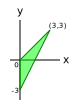
\includegraphics[width = 0.3\textwidth]{Test_bench_part_3x_images/Test_bench_part_3x_Solutions_image_8}
}
\end{tabular} \\
Therefore \(\sigma = \{(x,y) | 0 \leq x \leq 3 \;\text{and}\; 2x - 3 \leq y \leq x\}\)
\end{framed}}


%9
\dr{\begin{framed}
For \(\sigma = \left\{(r,\theta) \middle| 0 \leq \theta \leq \frac{\pi}{4} \;\text{and}\; 0 \leq r \leq 2\sin\theta\right\}\), \\
\begin{tabular}{cc}
\parbox{0.6\textwidth}{
The curve \(r = 2\sin\theta\) is equivalent to:
\begin{align*}
r = 2\sin\theta \iff & r = 2(y/r) 
\iff r^2 = 2y \\
\iff & x^2 + y^2 = 2y 
\iff x^2 + (y - 1)^2 = 1
\end{align*}
which is a circle centered on the point \((0,1)\) and has a radius of \(1\). The lower bound of \(\theta = 0\) generates the line \(y = 0\), while the upper bound of \(\theta = \frac{\pi}{4}\) generates the line \(y = x\). The portion of the aforementioned circle that is sandwiched between these two lines is shown on the right. 
} & \parbox{0.4\textwidth}{

\includegraphics[width = 0.3\textwidth]{Test_bench_part_3x_images/Test_bench_part_3x_Solutions_image_9}
}
\end{tabular} \\
Therefore \(\sigma = \{(x,y) | 0 \leq x \leq 1 \;\text{and}\; 1 - \sqrt{1 - x^2} \leq y \leq x\}\)
\end{framed}}

\pagebreak

%10
\dr{\begin{framed}
For \(\sigma = \left\{(r,\theta) \middle| -\atan(2) \leq \theta \leq \frac{\pi}{4} \;\text{and}\; 0 \leq r \leq \frac{2\cos\theta + \sin\theta}{\cos^2\theta}\right\}\), \\
\begin{tabular}{cc}
\parbox{0.6\textwidth}{
The curve \(r = \frac{2\cos\theta + \sin\theta}{\cos^2\theta}\) is equivalent to:
\begin{align*}
& r = \frac{2\cos\theta + \sin\theta}{\cos^2\theta} 
\iff r = \frac{2(x/r) + y/r}{(x/r)^2} \\ 
\iff & 1 = \frac{2x + y}{x^2} 
\iff y = x^2 - 2x
\end{align*}
which is a parabola with a turning point at \((1,-1)\) and which passes through \((0,0)\). The lower bound of \(\theta = -\atan(2)\) generates the line \(y = -2x\), while the upper bound of \(\theta = \frac{\pi}{4}\) generates the line \(y = x\).  The line \(y = 2x\) is tangent to the parabola at \((0,0)\), while the line \(y = x\) intersects the parabola at \((0,0)\) and \((3,3)\). The portion of the parabola that forms \(\sigma\) is shown on the right.
} & \parbox{0.4\textwidth}{

\includegraphics[width = 0.3\textwidth]{Test_bench_part_3x_images/Test_bench_part_3x_Solutions_image_10}
}
\end{tabular} \\
Therefore \(\sigma = \{(x,y) | 0 \leq x \leq 3 \;\text{and}\; x^2 - 2x \leq y \leq x\}\)
\end{framed}}


%11
\dr{\begin{framed}
For \(\sigma = \left\{(r,\theta) \middle| -\frac{\pi}{2} \leq \theta \leq \atan(\frac{3}{2}) \;\text{and}\; 0 \leq r \leq \frac{\sin\theta + \sqrt{1 + 3\cos^2\theta}}{2\cos^2\theta}\right\}\), \\
\begin{tabular}{cc}
\parbox{0.6\textwidth}{
The curve \(r = \frac{\sin\theta + \sqrt{1 + 3\cos^2\theta}}{2\cos^2\theta}\) is equivalent to: 
\begin{align*}
& r = \frac{\sin\theta + \sqrt{1 + 3\cos^2\theta}}{2\cos^2\theta} 
\iff r = \frac{y/r + \sqrt{1 + 3(x/r)^2}}{2(x/r)^2} \\
\iff & 1 = \frac{y + \sqrt{r^2 + 3x^2}}{2x^2} 
\iff 2x^2 = y + \sqrt{4x^2 + y^2} \\
\iff & 2x^2 - y = \sqrt{4x^2 + y^2} 
\iff 4x^4 - 4x^2y + y^2 = 4x^2 + y^2 \\
\iff & 4x^2y = 4x^4 - 4x^2 
\iff y = x^2 - 1
\end{align*}
The lower bound of \(\theta = -\frac{\pi}{2}\) generates the line \(x = 0\). The upper bound of \(\theta = \atan(\frac{3}{2})\) generates the line \(y = \frac{3}{2}x\). The line \(y = \frac{3}{2}x\) intersects the parabola \(y = x^2 - 1\) 
%\begin{align*}
%& \frac{3}{2}x = x^2 - 1 \iff x^2 - \frac{3}{2}x - 1 = 0 \\
%\iff & x = \frac{3/2 \pm \sqrt{9/4 + 4}}{2} 
%= \frac{3/2 \pm \sqrt{25/4}}{2} \\
%& \quad = \frac{3/2 \pm 5/2}{2} 
%= \frac{4,-1}{2} 
%= 2,-1/2
%\end{align*}
at the points \((2,3)\) and \((-1/2,-3/4)\), though only the point \((2,3)\) is relevant to \(\sigma\). \(\sigma\) is displayed on the right.
} & \parbox{0.4\textwidth}{

\includegraphics[width = 0.3\textwidth]{Test_bench_part_3x_images/Test_bench_part_3x_Solutions_image_11}
}
\end{tabular} \\
Therefore \(\sigma = \{(x,y) | 0 \leq x \leq 2 \;\text{and}\; x^2 - 1 \leq y \leq \frac{3}{2}x\}\)
\end{framed}}

\pagebreak

%12
\dr{\begin{framed}
For \(\sigma = \left\{(r,\theta) \middle| -\frac{\pi}{6} \leq \theta \leq \frac{\pi}{6} \;\text{and}\; 2\cos\theta - \sqrt{4\cos^2\theta - 3} \leq r \leq 2\cos\theta + \sqrt{4\cos^2\theta - 3}\right\}\), \\
The curve \(r = 2\cos\theta \pm \sqrt{4\cos^2\theta - 3}\) is equivalent to:
\begin{align*}
& r = 2\cos\theta \pm \sqrt{4\cos^2\theta - 3} 
\iff r = 2(x/r) \pm \sqrt{4(x/r)^2 - 3} \\
\iff & r^2 = 2x \pm \sqrt{4x^2 - 3r^2} 
\iff x^2 + y^2 = 2x \pm \sqrt{x^2 - 3y^2} \\
\iff & x^2 + y^2 - 2x = \pm \sqrt{x^2 - 3y^2} \\
\iff & x^4 + y^4 + 4x^2 + 2x^2y^2 - 4x^3 - 4xy^2 = x^2 - 3y^2 \\
\iff & y^4 + (2x^2 - 4x + 3)y^2 + (x^4 - 4x^3 + 3x^2) = 0 
\end{align*}
\begin{tabular}{cc}
\parbox{0.6\textwidth}{
using the quadratic formula gives:
\begin{align*}
\iff & y^2 = \frac{(-2x^2 + 4x - 3) \pm \sqrt{16x^2 - 24x + 9}}{2} \\
\iff & y^2 = \frac{(-2x^2 + 4x - 3) \pm (4x - 3)^2}{2} \\
\iff & y^2 = -x^2 + 4x - 3, -x^2
\end{align*}
since \(y^2 \geq 0\), the option of \(y^2 = -x^2\) is not allowed. Therefore:
\begin{align*}
& y^2 = -x^2 + 4x - 3 
\iff (x - 2)^2 + y^2 = 1
\end{align*}
which is a circle centered on the point \((2,0)\) with a radius of \(1\). The lower bound of \(\theta = -\frac{\pi}{6}\) gives the line \(y = -\frac{x}{\sqrt{3}}\). The upper bound of \(\theta = \frac{\pi}{6}\) gives the line \(y = \frac{x}{\sqrt{3}}\). Both lines \(y = -\frac{x}{\sqrt{3}}\) and \(y = \frac{x}{\sqrt{3}}\) intersect the circle at exactly one point and are therefore tangent to the circle, and do not clip the circle. \(\sigma\) is shown on the right.
} & \parbox{0.4\textwidth}{
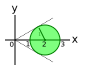
\includegraphics[width = 0.4\textwidth]{Test_bench_part_3x_images/Test_bench_part_3x_Solutions_image_12}
}
\end{tabular} \\
Therefore \(\sigma = \{(x,y) | 1 \leq x \leq 3 \;\text{and}\; -\sqrt{1 - (x-2)^2} \leq y \leq \sqrt{1 - (x-2)^2}\}\)
\end{framed}}





%%%%%%%%%%%%%%%%%% QUESTION 3
\section*{Question 3:}

For the following iterated integrals, reverse the order of integration:

\begin{itemize}
\item \(\int_{x = 0}^2 \int_{y = x^2}^{2x} f(x,y)dydx\)
\item \(\int_{y = 0}^3 \int_{x = -\sqrt{9 - y^2}}^{\sqrt{9 - y^2}} f(x,y)dxdy\)
\item \(\int_{x = -5}^1 \int_{y = -4}^{-x^2 - 4x + 1} f(x,y)dydx\)
\end{itemize}


%%%%%%%%%%%%%%%%%% SOLUTION 3

\vspace{5mm}
\dr{\textbf{Solution:}}

%13
\dr{\begin{framed}
For \(\int_{x = 0}^2 \int_{y = x^2}^{2x} f(x,y)dydx\), \\
the region of integration is: \(\sigma = \{(x,y) | 0 \leq x \leq 2 \;\text{and}\; x^2 \leq y \leq 2x\}\) \\
\begin{tabular}{cc}
\parbox{0.6\textwidth}{
The line \(y = 2x\) and the parabola \(y = x^2\) intersect at the points \((0,0)\) and \((2,4)\). These points form the ``endpoints" of \(\sigma\). The line \(y = 2x\) can be rearranged to give \(x = y/2\). The parabola \(y = x^2\) can be arranged to give \(x = \pm \sqrt{y}\), and since \(x \geq 0\), only \(x = \sqrt{y}\) matters. The region \(\sigma\) is shown on the right.
} & \parbox{0.4\textwidth}{

\includegraphics[width = 0.2\textwidth]{Test_bench_part_3x_images/Test_bench_part_3x_Solutions_image_13}
} 
\end{tabular} \\
Therefore \(\sigma = \{(x,y) | 0 \leq y \leq 4 \;\text{and}\; y/2 \leq x \leq \sqrt{y}\}\) \\ 
and \(\int_{x = 0}^2 \int_{y = x^2}^{2x} f(x,y)dydx = \int_{y = 0}^4 \int_{x = y/2}^{\sqrt{y}} f(x,y)dxdy\)
\end{framed}}


%14
\dr{\begin{framed}
For \(\int_{y = 0}^3 \int_{x = -\sqrt{9 - y^2}}^{\sqrt{9 - y^2}} f(x,y)dxdy\), \\
the region of integration is: \(\sigma = \{(x,y) | 0 \leq y \leq 3 \;\text{and}\; -\sqrt{9-y^2} \leq x \leq \sqrt{9-y^2}\}\) \\
\begin{tabular}{cc}
\parbox{0.6\textwidth}{
\(\sigma\) is a semicircle with a radius of \(3\) that is centered at \((0,0)\) and is above the line \(y = 0\). \(\sigma\) is shown on the right.
} & \parbox{0.4\textwidth}{
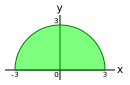
\includegraphics[width = 0.3\textwidth]{Test_bench_part_3x_images/Test_bench_part_3x_Solutions_image_14}
} 
\end{tabular} \\
Therefore \(\sigma = \{(x,y) | -3 \leq x \leq 3 \;\text{and}\; 0 \leq y \leq \sqrt{9 - x^2}\}\) \\
and \(\int_{y = 0}^3 \int_{x = -\sqrt{9 - y^2}}^{\sqrt{9 - y^2}} f(x,y)dxdy = \int_{x = -3}^3 \int_{y = 0}^{\sqrt{9 - x^2}} f(x,y)dydx\)
\end{framed}}

\pagebreak

%15
\dr{\begin{framed}
For \(\int_{x = -5}^1 \int_{y = -4}^{-x^2 - 4x + 1} f(x,y)dydx\), \\
the region of integration is: \(\sigma = \{(x,y) | -5 \leq x \leq 1 \;\text{and}\; -4 \leq y \leq -x^2 - 4x + 1\}\) \\
\begin{tabular}{cc}
\parbox{0.6\textwidth}{
\(\sigma\) is bounded from below by the line \(y = -4\), and from above by the parabola \(y = -x^2 - 4x + 1\). The line and parabola intersect at the points \((-5,-4)\) and \((1,-4)\), which matches exactly the given range for \(x\). Region \(\sigma\) is shown on the right. The equation \(y = -x^2 - 4x + 1\) is equivalent to:
\begin{align*}
& y = -x^2 - 4x + 1 
\iff y = -(x + 2)^2 + 5 \\
\iff & x = -2 \pm \sqrt{5 - y}
\end{align*} 
The minimum value of \(y\) is \(-4\), while the maximum value of \(y\) is \(5\). 
} & \parbox{0.4\textwidth}{
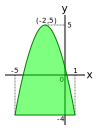
\includegraphics[width = 0.3\textwidth]{Test_bench_part_3x_images/Test_bench_part_3x_Solutions_image_15}
}
\end{tabular} \\
Therefore \(\sigma = \{(x,y) | -4 \leq y \leq 5 \;\text{and}\; -2 - \sqrt{5 - y} \leq x \leq -2 + \sqrt{5 - y}\}\) \\
and \(\int_{x = -5}^1 \int_{y = -4}^{-x^2 - 4x + 1} f(x,y)dydx = \int_{y = -4}^5 \int_{x = -2 - \sqrt{5 - y}}^{-2 + \sqrt{5 - y}} f(x,y)dxdy\)
\end{framed}}


\end{document}










